
\documentclass[a4paper]{article}



%%TikZ Begin - for diagrams 
\usepackage{pgf}
\usepackage{tikz}

\title{Example Usage}

\begin{document}

\maketitle

\begin{figure}[h]%

\centering







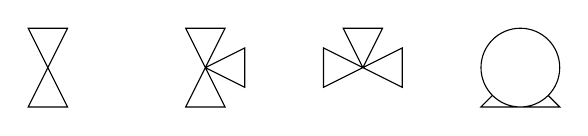
\begin{tikzpicture}


%% Shapes are always 2x their defined size value, I.e. a \TikZValveSize = 0.5 leads to a total valve height of 1
%% The default setting for elements is to have a span of ``1'' across the connecting sides.
%% elements can be rotated using the ``rotate around={angle:(point)}'' keyword, use in 90 degree steps is advised
%% While the rotate option may be inconvenient, it avoids the clutter of requiring multiples of every shape

\def\TikZValveSize{0.5} 
\def\TikZPumpSize{0.5} %%% helper value for ``base'' 0.3

\def\TikZValve{%
		++(-\TikZValveSize/2,\TikZValveSize) -- ++(\TikZValveSize,0) -- ++(-\TikZValveSize,-2*\TikZValveSize) -- ++(\TikZValveSize,0) -- cycle 
}

\def\TikZThreeWayValve{%
		-- ++(-\TikZValveSize/2*1,\TikZValveSize) -- 		++(\TikZValveSize,0) -- ++(-\TikZValveSize,-2*\TikZValveSize) -- ++(\TikZValveSize,0) -- ++(-\TikZValveSize/2,\TikZValveSize) %
		-- ++(\TikZValveSize,\TikZValveSize/2) -- ++(0,-\TikZValveSize) -- ++(-\TikZValveSize,\TikZValveSize/2) %-- cycle 
}

\def\TikZPump{%
		circle (\TikZPumpSize)
		++(-\TikZPumpSize,-\TikZPumpSize) ++(\TikZPumpSize*0.3,\TikZPumpSize*0.3) 
		-- ++(-\TikZPumpSize*0.3,-\TikZPumpSize*0.3) -- ++(2*\TikZPumpSize,0) -- ++(-\TikZPumpSize*0.3,\TikZPumpSize*0.3) 
}


%% Example Use

\draw (1,1) \TikZValve ;

\draw (3,1) \TikZThreeWayValve ;

\draw[rotate around={90:(5,1)}] (5,1) \TikZThreeWayValve ;

\draw (7,1) \TikZPump ;


\end{tikzpicture}





\end{figure}

\end{document}
